\chapter{Experiment 1: Supplementary Materials and methods}

\subsection*{Experimental Design}
\label{sec:supp_Experimental_Design}

\noindent This section describes how the display sequence of the 
oriented gratings in both the hemifields were generated per experimental run.
Independent sequences were generated per hemifield with equal number of occurences of
each orientation. There were 4 different orientations (0\textdegree,
45\textdegree, 90\textdegree, or 135\textdegree) each occuring for 
5 times in the sequence, contributing to 20 trials in one run.
The sequences were randomly shuffled per hemifield. in this analysis a 
single GLM was used to model the events in both the hemifields. This was done 
to account for potential interhemispheric cross-talk due to the 
simultaneous bilateral stimulation. Moreover, in order to minimize 
undesired attention shift effects, a simultaneous onsets of the stimulation 
in both hemifields was opted for. Combined with the further aspect of 
presenting the same number of stimulation trials per orientation in both hemifields, 
this unavoidably led to a singularity of the GLM design matrix, 
unless a further source of temporal variability was introduced.
In order to address this issue unilateral stimulation events (termed NULL events) 
was introduced. For the same reason NULL events were included in the analysis, 
as their exclusion would make the design matrix status as singular. However, 
it was possible to analyze these data using two separate models for the hemifields. 
In this scenario it was also possible to exclude NULL events from the design. 
This resulted in an overall improved classification performance, but did 
not impact the structure of the relative performance differences 
between resolutions (\mm{0.8}: 32.32\%, \mm{1.4}:41.78\%, \mm{2.0}: 46.42\%, and \mm{3.0}: 40.17\%)
Figure~\ref{fig:ipsi}A and Figure~\ref{fig:ipsi}B quantify how the NULL events decorrelate the 
stimulation between hemifields. The events with single hemifield stimulation 
were included in the analysis as shown in Figure~\ref{fig:ipsi}C. 





\begin{figure} \centering
  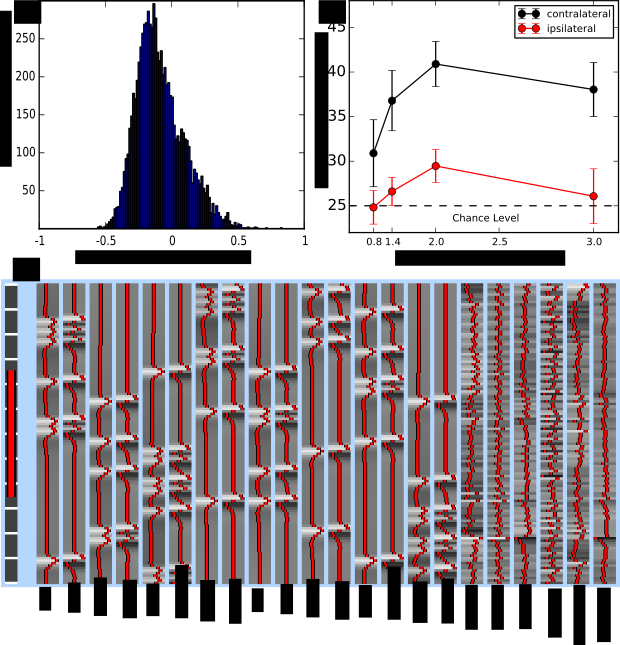
\includegraphics[width=\linewidth]{supplementary_figure_1}
  \caption{     \textbf{(A)} Histogram of paiwrise correlation (Spearman's Rank Correlation 
    Coefficient) between the 8 regressors corresponding to the events 
    occuring in both hemifields across subjects and scanning sessions. 
    \textbf{(B)} Orientation decoding accuracy on spatially unfiltered data 
    across acquisition resolutions in both contra-lateral and ipsi-lateral 
    V1 ROI. The ipsi-lateral accuracies show similar trend as the contra-lateral
    accuracies. The ipsi-lateral accuracies for \mm{1.4} and \mm{2} resolution show 
    low decoding performance and the \mm{0.8} and \mm{3} decoding accuracies 
    are at chance level. \textbf{(C)} Design matrix of one particular experimental run.
    There are 8 regressors for stimulation events in both hemifields 
    and 8 regressors more for the corresponding temporal derivatives. For 
    example LH\_0 regressor represents events of 0\textdegree gratings in 
    the left hemifield and LH\_0' is the corresponding temporal derivative.
    The motion parameters along 6 axes (motin\_x, motion\_y, motion\_z, 
    motion\_roll, motion\_pitch and motion\_yaw) are also included to model 
    the residual motion. 
  }

    \label{fig:ipsi}
\end{figure}


\subsection*{Spatial Filtering restricted to V1 ROI}


In Figure~\ref{fig:spatial_smoothing} the performance of orientation decoding was quantified following 
low-pass, high-pass, band-pass, and  band-stop spatial filtering in order to study 
the spatial frequency dependent orientation selective responses. All spatial filtering 
procedures were volumetric, using 3D Gaussian kernels and  ROI voxel 
selection was performed after spatial filtering with different Gaussian kernel widths 
on the entire volume. Though this 3D filtering procedure was 
being extensively used in previous studies like \citep{opdebeeck_2010, swisher_2010}, 
this approach causes partial volume effects with information from adjacent bits of 
cortex, signals from white matter and superficial vessels, and, as demonstrated 
in Figure~\ref{fig:distance_plot}, even with signals recorded in the two banks of  
the calcarine sulcus, with the 'matching' kernel width, all of which 
can contribute to decoding. This confounds filter width with the 
extent of the cortical region from which information is drawn. To avoid 
this confoundation, 2 additional spatial filtering approaches were adopted, namely
Smoothing with missing values Figure~\ref{fig:surface_ecs} A-D and surface-based 
smoothing Figure~\ref{fig:surface_ecs} E-H.
  
\paragraph*{Smoothing with missing values}
Similar to the spatial filtering procedure performed in \citet{alink_2013}, 
the voxel values outside the V1 ROI were considered to be missing values (NaN)
instead of applying spatial filtering on the whole volume, prior to any masking.
To reduce the effect of smoothing across hemispheres with large Gaussian kernels,
this technique of smoothing was restricted to individual hemispheres. First, 
voxel values outside the left V1 ROI was considered to be NaNs and
spatial smoothing was applied. The same procedure was applied to the right ROI, 
and then the smoothed left and right V1 ROI were added to form the smoothed 
BOLD volume. The same nested cross validation approach was performed on the 
smoothed data. The results of this analyis is shown in Figure~\ref{fig:surface_ecs} A-D.  

\paragraph*{Surface based smoothing}
In this approach, Freesurfer \texttt{mri\_vol2surf} function \citep{dale_1999} 
was used with \texttt{surf-fwhm} parameter on the BOLD images to 
obtain a smoothed cortical surface corresponding to a particular 
gaussian kernel. In the next step this smoothed surface was mapped into 
the BOLD volumetric space with Freesurfer \texttt{mri\_surf2vol} function 
with tri-linear interpolation and \texttt{fill-projfrac} parameter 
ranging from 0-1 in steps of 0.01 projected on the white surface. This 
procedure was performed per hemisphere reducing the cross-hemisphere smoothing effects. 
The same nested cross validation approach was performed on the 
smoothed data. The results of this analyis is shown in Figure~\ref{fig:surface_ecs} E-H.
The results of surface based smoothing were similar to those of the 3D Gaussian filter, 
but the decoding accuracy did not decrease rapidly with greater filtering. 
This surface-based smoothing approach reduced the partial voluming effects of 3D filters, 
which included contributions from gray matter voxels together with 
white matter and space outside the brain adding to the noise. 
The band pass filtering peak was present at 5-8mm but less pronounced 
more evenly sloped than what was obtained from volumetric filtering.


\begin{figure} \centering
  \includegraphics[width=\linewidth]{supplementary_figure_2}
  \caption{
    %
	TODO
   %
  }

    \label{fig:surface_ecs}
\end{figure}


\subsection*{Resampling to other resolutions}

Resampling method from one resolution to the other was a 2 step procedure. 
Here it is explained with the example of resampling a \mm{0.8} isotropic 
data to a \mm{3.0} isotropic data. First Fast Fourier Transform based spatial filtering was 
performed on the distortion corrected \mm{0.8} iso data (see Figure~\ref{fig:resample_r08_r30}A)
using the scipy function \texttt{signal.resample()}. This removed the higher frequency 
components but the voxel size remained \mm{0.8} iso with in-plane matrix 
size (208, 160) with 32 slices (see Figure~\ref{fig:resample_r08_r30}B). 
In the next step, affine resampling or reslicing was performed with 
nilearn implementation \texttt{resample\_img()} method to convert 
the fft filtered image to the corresponding \mm{3.0} iso voxel size. 
The in-plane matrix size became (66, 66) with 37 slices similar to the 
acquired \mm{3.0} data.

\begin{figure} \centering
  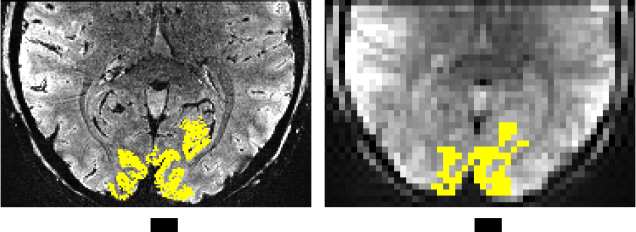
\includegraphics[width=\linewidth]{supplementary_figure_3}
  \caption{
    %
	Resampling from 0.8mm iso to 3.0mm iso resolution (A) Distortion 
    corrected 0.8mm isotropic BOLD image overlayed with V1 ROI mask. 
    (B) Removal of high-frequency components using scipy function signal.resample() 
    overlayed with resampled V1 ROI mask (linear interpoltion using 
    scipy function ndimage.interpolation.zoom())
   %
  }

    \label{fig:resample_r08_r30}
\end{figure}


\section*{Supplementary Figures}

\begin{figure} \centering
  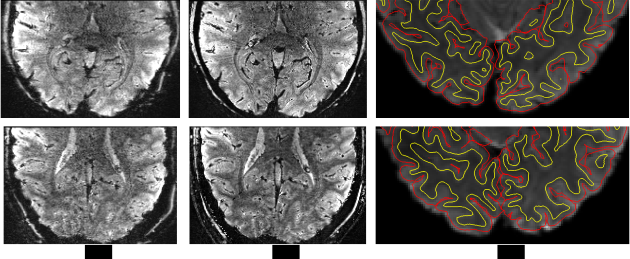
\includegraphics[width=\linewidth]{supplementary_figure_4}
  \caption{
    %
	The alignment of distortion corrected EPI functional data obtained at 7 
	Tesla to the structural data obtained at 3 Tesla from 2 subjects. 
	(A) Uncorrected data from Siemens 7T Magnetom 
	(B) Distortion corrected data \citep{in_2012}
	(C) Alignment of the EPI sequences acquired in 7T to 
	the corresponding 3T Structural images. The white matter 
	segmentation is shown with yellow lines and pial surface with red 
	lines. The white matter and pial surface segmentations were 
	performed on the structural data with Freesurfer and overlayed on 
	the aligned EPI images to show the quality of the alignments.   
   %
  }
\end{figure}



\begin{figure} \centering
  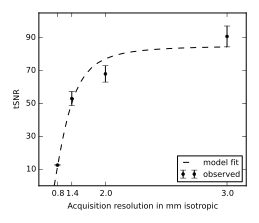
\includegraphics[width=0.5\linewidth]{supplementary_figure_5}
  \caption{
    %
	tSNR as a function of voxel volume. The observed data are represented by dots
    and the errorbars represent the SEM across subjects. The dashed line shows the fit
    to the following model $\text{tSNR}=\kappa  V / \sqrt{1+\lambda^2  \kappa^2  V^2}$ 
    similar to the report of \citet{triantafyllou_2005}
   %
  }
  \label{fig:tSNR_vs_resolution}
\end{figure}

